\documentclass[twocolumn,superscriptaddress,pre]{revtex4-1}

\usepackage[english]{babel}
\usepackage[utf8]{inputenc}
\usepackage{prettyref}
\usepackage{graphicx}
\usepackage{amsmath}
\usepackage{amssymb}

\usepackage[babel]{csquotes}
\usepackage[hidelinks]{hyperref} % load as last package

\DeclareMathOperator{\atan}{atan}


\begin{document}

\title{Casimir force between metallic mirrors}

\author{Michael Hartmann}
\affiliation{Universität Augsburg, Institut für Physik, 86135 Augsburg, Germany}

\date{\today}

\begin{abstract}
The Casimir free energy after Wick rotation depends on the dielectric function
on the imaginary axis. Here, we discuss how the dielectric function can be
rotated to the imaginary axis.
\end{abstract}

\maketitle

\section{Introduction}

The Casimir free energy in the plane-plane geometry is a function of the
separation $L$ between both plates, the temperature $T$ and the optical
properties of the plates
\begin{equation}
{\cal F} = {\cal F}\left(L,T,\epsilon(i\omega)\right) \,.
\end{equation}
Due to the Wick rotation, the dielectric function is evaluated on the imaginary
axis. The dielectrict function on the imaginary axis is connected with the
imaginary part of the dielectric function by the Kramers-Kronig relations.

Here, we show how to compute the dielectric function on the imaginary axis from
optical data, and discuss problems of this procedure. A more detailled discussion
can be found in \cite{Lambrecht2000}.

\section{Kramers-Kronig relations}

\begin{figure}
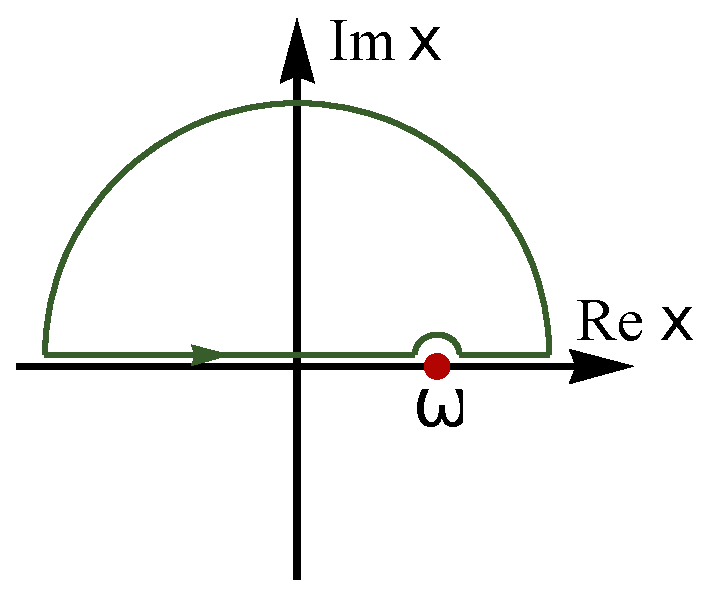
\includegraphics[width=0.5\columnwidth]{img/contour.eps}
\caption{Contour $\cal C$ used to derive the Kramers-Kronig relations.}
\label{fig:contour}
\end{figure}

The Kramers-Kronig relations connect the real and imaginary parts of a complex
function that is analytic in the upper half-plane. Let $\chi=\chi'+i\chi''$ be
analytic in the closed upper half-space, $\chi'$ and $\chi''$ are real, and
$\chi(x)$ vanishes faster than $|x|^{-1}$ as $x\to\infty$. Then the line
integral with the contour $\cal C$ sketched in Fig. \ref{fig:contour} vanishes,
\begin{equation}
\oint_{\cal C} \mathrm{d}x \frac{\chi(x)}{x-\omega} = \lim_{\epsilon\to0^+} \int_{-\infty}^\infty \mathrm{d}x \frac{\chi(x)}{x-\omega+i\epsilon} = 0 \,.
\end{equation}
Substituting $z=x-\omega$ and separating real and imaginary parts, we find
\begin{equation}
0 = \lim_{\epsilon\to0^+}\int_{-\infty}^\infty \mathrm{d}z \frac{z \chi(z+\omega)}{z^2+\epsilon^2} - i\pi \lim_{\epsilon\to0^+} \int_{-\infty}^\infty \mathrm{d}z \frac{\epsilon \chi(z+\omega)}{\pi(z^2+\omega^2)} \,.
\end{equation}
The first term on the right-hand side corresponds to a principal value, while
the second term in the limit $\epsilon\to0^+$ becomes a delta-function. Thus we find
\begin{equation}
0 = {\cal P} \int_{-\infty}^\infty \mathrm{d}z \frac{\chi(z+\omega)}{z} - i\pi \chi(\omega),
\end{equation}
which after resubstituition $x$ and splitting up real and imaginary parts,
yields the famous Kramers-Kronig relations:
\begin{align}
\label{eq:KK1}
\chi'(\omega)  &= +\frac{1}{\pi} {\cal P} \int_{-\infty}^\infty \mathrm{d}x \frac{\chi''(x)}{x-\omega} \\
\label{eq:KK2}
\chi''(\omega) &= -\frac{1}{\pi} {\cal P} \int_{-\infty}^\infty \mathrm{d}x \frac{\chi'(x) }{x-\omega}
\end{align}


\section{Rotating $\epsilon(\omega)$ to the imaginary axis}

Here, we focus on the dielectric function
\begin{equation}
\epsilon(\omega)=\chi(\omega)+1 \,.
\end{equation}
As $\epsilon(t)$ is real, $\epsilon(-\omega) = \epsilon^*(\omega)$, and
$\epsilon'(\omega)$ is an even function while $\epsilon''(\omega)$ is an odd
function. Using the Kramers-Kronig relation \eqref{eq:KK2}, we find that the
imaginary part of $\epsilon(i\omega)$ vanishes, because the integrand is odd
with respect to $x$,
\begin{equation}
\epsilon''(i\omega) = - \frac{1}{\pi} \int_{-\infty}^\infty \mathrm{d}x \frac{\epsilon'(x)-1}{x-i\omega} = 0 \,.
\end{equation}
The real part is readily evaluated using \eqref{eq:KK1}
\begin{equation}
\epsilon'(i\omega)-1 = \frac{1}{\pi} \int_{-\infty}^\infty \mathrm{d}x \frac{x\epsilon''(x)}{x^2+\omega^2} + \frac{i\omega}{\pi} \int_{-\infty}^\infty \mathrm{d}x \frac{\epsilon''(x)}{x^2+\omega^2} \,. 
\end{equation}
The integrand of the first integral on the right-hand side is even, the second integral vanishes, because the integrand is odd. Thus, we find
\begin{equation}
\epsilon(i\omega)-1 = \frac{2}{\pi} \int_0^\infty \mathrm{d}x \frac{x\epsilon''(x)}{x^2+\omega^2}
\end{equation}
for the dielectric function on the imaginary axis.

So, the dielectric function on the imaginary axis $\epsilon(i\omega)$ can be
computed from the imaginary part of $\epsilon''(\omega)$. However,
$\epsilon''(\omega)$ is only available in a finite interval
$\omega_\mathrm{min} \le \omega \le \omega_\mathrm{max}$. Typical values are $\omega_\mathrm{min} \sim 0.05\,$eV
and $\omega_\mathrm{max} \sim 10^4\,$eV, where $1\,$eV$=1.537\,$rad/s.
We split up the
integral in three contributions and discuss each integral separately:
\begin{align}
\nonumber
\epsilon(i\omega)-1 =&
\frac{2}{\pi} \int_0^{\omega_\mathrm{min}} \mathrm{d}x \frac{x\epsilon''(x)}{x^2+\omega^2} +
\frac{2}{\pi} \int_{\omega_\mathrm{min}}^{\omega_\mathrm{max}} \mathrm{d}x \frac{x\epsilon''(x)}{x^2+\omega^2} \\
&+\frac{2}{\pi} \int_{\omega_\mathrm{max}}^\infty \mathrm{d}x \frac{x\epsilon''(x)}{x^2+\omega^2} \equiv I_1 + I_2 + I_3
\end{align}

\begin{itemize}
\item As $\epsilon''(\omega_\mathrm{max}) \sim 5\times10^{-6}$, the contribution
from $I_3$ is negligible.
\item Integral $I_2$ can be evaluated using numerical quadrature. Typically,
many points are available and the integration yields no problems. For example,
one might use Simpson quadrature.
\item Integral $I_1$ cannot be evaluated numerically, because no data is
available and one must rely on extrapolation. The dielectric functions of good
metals like gold are well described by the Drude model
\begin{equation}
\label{eq:drude}
\epsilon^D(\omega) = 1 - \frac{\omega_P^2}{\omega(\omega+i\gamma)},
\end{equation}
where $\omega_P \sim 9\,$eV is the Plasma frequency and $\gamma \sim 35\,$meV
is related to dissipation. Using the Drude model to extrapolate the data, the
integral becomes
\begin{equation}
I_3 = \frac{2}{\pi} \frac{\omega_P^2}{\omega^2-\gamma^2} \left[ \atan\left(\frac{\omega_\mathrm{min}}{\gamma}\right) - \frac{\gamma}{\omega} \atan\left(\frac{\omega_\mathrm{min}}{\omega}\right)\right] \,.
\end{equation}
Please note that the value of this integral depends sensitively on the plasma
frequency $\omega_P$.
\end{itemize}

\section{Optical data}

\begin{table}
\begin{center}
\begin{tabular}{|ll|l|l|}
\hline
source & preparation & $\omega_P$ (eV) & $\gamma$ (meV) \\
\hline
\hline
Palik & & $9$ & $30$ \\
\hline
Svetovoy & $400\,$nm/Si & $6.82\pm0.08$ & $40.5\pm2.1$ \\
         & $200\,$nm/Si & $6.83\pm0.15$ & $39.5\pm4.4$ \\
         & $100\,$nm/Si & $7.84\pm0.07$ & $49.0\pm2.1$ \\
         & $120\,$nm/Si & $8.00\pm0.16$ & $35.7\pm5.1$ \\
         & $120\,$nm/mica & $8.38\pm0.08$ & $37.1\pm1.9$ \\
\hline
Olmon & EV & $8.5\pm0.5$ & $47$ \\
Olmon & TS & $8.8\pm0.05$ & $50$ \\
Olmon & SC & $8.1\pm0.8$ & $47$ \\
\hline
\end{tabular}
\end{center}
\caption{Plasma frequency $\omega_P$ and dissipation $\gamma$ for gold with
different preparation. The data is given by \cite{Palik1995,Olmon2012,Svetovoy2008}.
The values for $\omega_P$ and $\gamma$ for Palik were obtained in \cite{Lambrecht2000}.}
\label{tab:gold}
\end{table}

\begin{figure}
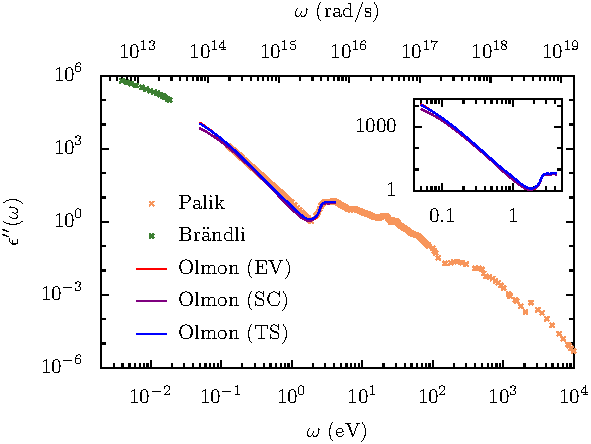
\includegraphics[width=0.95\columnwidth]{img/eps.pdf}
\caption{Imaginary part of the dielectric function $\epsilon(\omega)$ for the
data of Palik \cite{Palik1995}, and the experiments by Olmon \cite{Olmon2012}
and Bennet \cite{Bennett1966}.}
\label{fig:eps}
\end{figure}

\begin{figure}
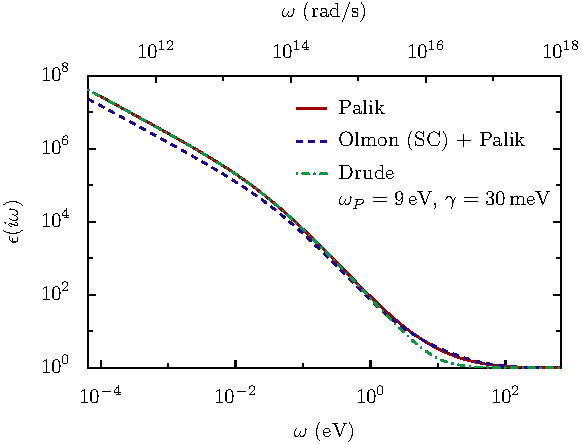
\includegraphics[width=0.95\columnwidth]{img/eps_imag.pdf}
\caption{Dielectric function for imaginary frequencies, $\epsilon(i\omega)$.}
\label{fig:eps_imag}
\end{figure}

\begin{figure}
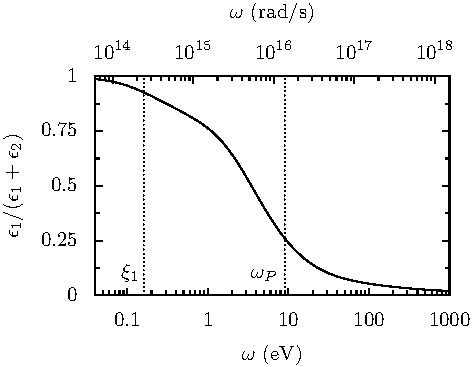
\includegraphics[width=0.7\columnwidth]{img/ratio.pdf}
\caption{Ratio of the integral $I_1$ by the total contribution $I_1+I_2$. The contribution of $I_3$ is negligibly small.}
\label{fig:ratio}
\end{figure}

\begin{figure}
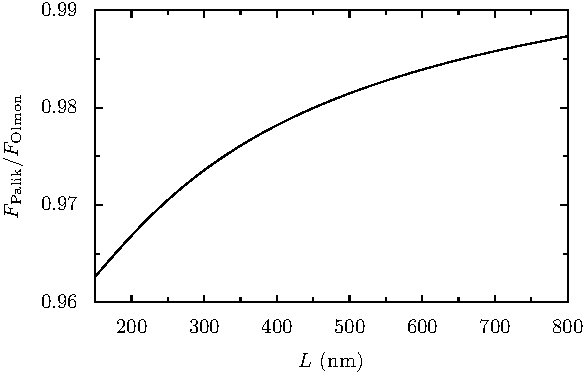
\includegraphics[width=0.7\columnwidth]{img/diff.pdf}
\caption{Ratio of the force (PFA) for $R=100\,\mu$m and $T=300\,$K using the optical data from Palik \cite{Palik1995} and Olmon \cite{Olmon2012}.}
\label{fig:diff}
\end{figure}

There are many different experiments that measured the dielectric function of
gold. Often, the handbook data edited by \textsc{Palik} is used.
\cite{Palik1995}. \textsc{Olmon} et al.\ measured the optical properties of
evaporated (EV, 200\,nm thick film deposited by evaporation onto a soda-lime
glass substrate), template-stripped (TS, 200\,nm film deposited onto a clean
silicon substrate in the same evaporation run), and single-crystal Au(111) (SC,
thickness 1\,mm, diameter 10\,mm) gold in the range from 0.04 to 4.14\,eV
\cite{Olmon2012}. \textsc{Svetovoy} et al.\ measured five gold films prepared
by Au deposition on cleaned (100) Si or mica substrate with varying thickness
\cite{Svetovoy2008}.

The imaginary part of the dielectric function, $\epsilon''(\omega)$ for the
data by Palik \cite{Palik1995} and the experiments by Olmon et al.\
\cite{Olmon2012} and Bennett et al.\ \cite{Bennett1966} is listed in Fig.
\ref{fig:eps}. The dielectric function for imaginary frequencies is plotted in
Fig. \ref{fig:eps_imag}. The obtained functions differ depending on which
optical data were used. The simple Drude model \eqref{eq:drude} is in good
agreement with the dielectric function obtained by the optical data up to
frequencies of $\sim 1\,$eV when interband transitions become important.

Interestingly, the experiments find rather different values for the plasma
frequency $\omega_P$ and the dissipation rate $\gamma$, see Table
\ref{tab:gold}. As the value of $I_1$ depends sensitively on the value of the
plasma frequency, high accuracy in Casimir experiments need a good knowledge
of the plasma frequency. In particular, low Matsubara frequencies depend
strongly on the extrapolation, because for such frequencies the contribution
of $I_1$ is dominant, as can be seen in Fig. \ref{fig:ratio}.

In the computation of the Casimir force, using different optical data may add
up to a difference of several percent. In Fig. \ref{fig:diff} we show the ratio of
Casimir force for a radius $R=100\,\mu$m and room-temperature $T=300\,$K using the
dielectric function obtained by Palik, and a combination of Olmon for small and Palik
at high frequencies. The difference of both dielectric functions is quite big, because
the plasma frequency for Palik is $\omega_P=9\,$eV, and for Olmon it is $\omega_P=8.45\,$eV.


\section{Window functions}

One way proposed by \textsc{Bimonte} \cite{Bimonte2010} to circumvent the high contribution
of $I_1$ is to alter the Kramers-Kronig relations by a window function $f(x)$. More precisely,
using the same derivation as before for $\chi(x)=f(x)[\epsilon(x)-1]$ one finds
\begin{equation}
\epsilon(i\omega)-1 = \frac{2}{\pi f(i\omega)} \int_0^\infty \mathrm{d}x \frac{x}{x^2+\omega^2} \mathrm{Im}\left\{ f(x)\left[\epsilon(x)-1\right] \right\} \,.
\end{equation}
The window function $f(x)$ can now be chosen in such a way that is suppresses
the contributions to $I_1$. However, it was pointed out in \cite{Shpak2011}
that the use of a window function can in some cases distort the Casimir force
calculations.

\section{Conclusion}

The dielectric function at imaginary frequencies $\epsilon(i\omega)$ depends on
the optical data used. The optical data, on the other hand, strongly depends on
the preparation. The plasma frequency may range from about about 8 to $9\,$eV
which gives a very different contribution from $I_1$. The difference may yield
to a deviation of several percent in the Casimir force.

\begin{thebibliography}{99}

\bibitem{Lambrecht2000}
A. Lambrecht and S. Reynaud,
Casimir force between metallic mirrors,
Eur. Phys. J. D. \textbf{8}, 309-318 (2000).

\bibitem{Palik1995}
In \textit{Handbook of Optical Constants of Solids},
edited by E. D. Palik (Academic Press, New York, 1995)

\bibitem{Olmon2012}
R. L. Olmon, B. Slovick, T. W. Johnson, D. Shelton, S-H Oh, G. D. Boreman, and M. B. Raschke,
Optical dielectric function of gold,
Phys. Rev. B \textbf{86}, 235147 (2012)

\bibitem{Svetovoy2008}
V. B. Svetovoy, P. J. van Zwol, G. Palasantzas, and J. Th. M. De Hosson,
Optical properties of gold films and the Casimir force,
Phys. Rev. B. \textbf{77}, 035439 (2008)

\bibitem{Bennett1966}
H. E. Bennett and J. M. Bennett,
Optical Properties and Electronic Structure of Metals and Alloys edited by F. Abeles (North-Holland, Amsterdam, 1966), p. 175

\bibitem{Bimonte2010}
G. Bimonte,
Generalized Kramers-Kronig transform for Casimir effect computations,
Phys. Rev. A. \textbf{81}, 062501 (2010)

\bibitem{Shpak2011}
O. Shpak and G. Pasantzas,
Analysis of Casimir force with window functions: Kramers-Kronig general approach for real measured dielectric data,
Phys. rev. A. \textbf{84}, 044501 (2011)

\end{thebibliography}

\end{document}
